\chapter{Developmental stability of the \mrna--\trna interface}

In order to study how changes in \mrna gene expression relate to changes in
\trna gene expression, we collected tissue samples from six time points in mouse
development: two before birth (E15.5 and E18.5, which stands for \num{15.5} and
\num{18.5} days after gestation of the oocyte, respectively); two shortly after
birth, happening around E20 (P0.5 and P4 --- \num{0.5} and \num{4} days after
birth, respectively) and two after weaning the juvenile mice (P22 and P29).

For each of these time points, tissue was collected from whole liver and whole
brain (homogenised) and prepared for \rnaseq and \pol3 \chipseq in order to
assay \mrna and \trna gene expression. \Cref{fig:trna-project-outline}
summarises the experimental procedure.\footnote{The wet-lab work of this project
was performed by Bianca Schmitt.}
\todo{Remove background gradients from graphics}

\begin{figure}[h!]
    \centering
    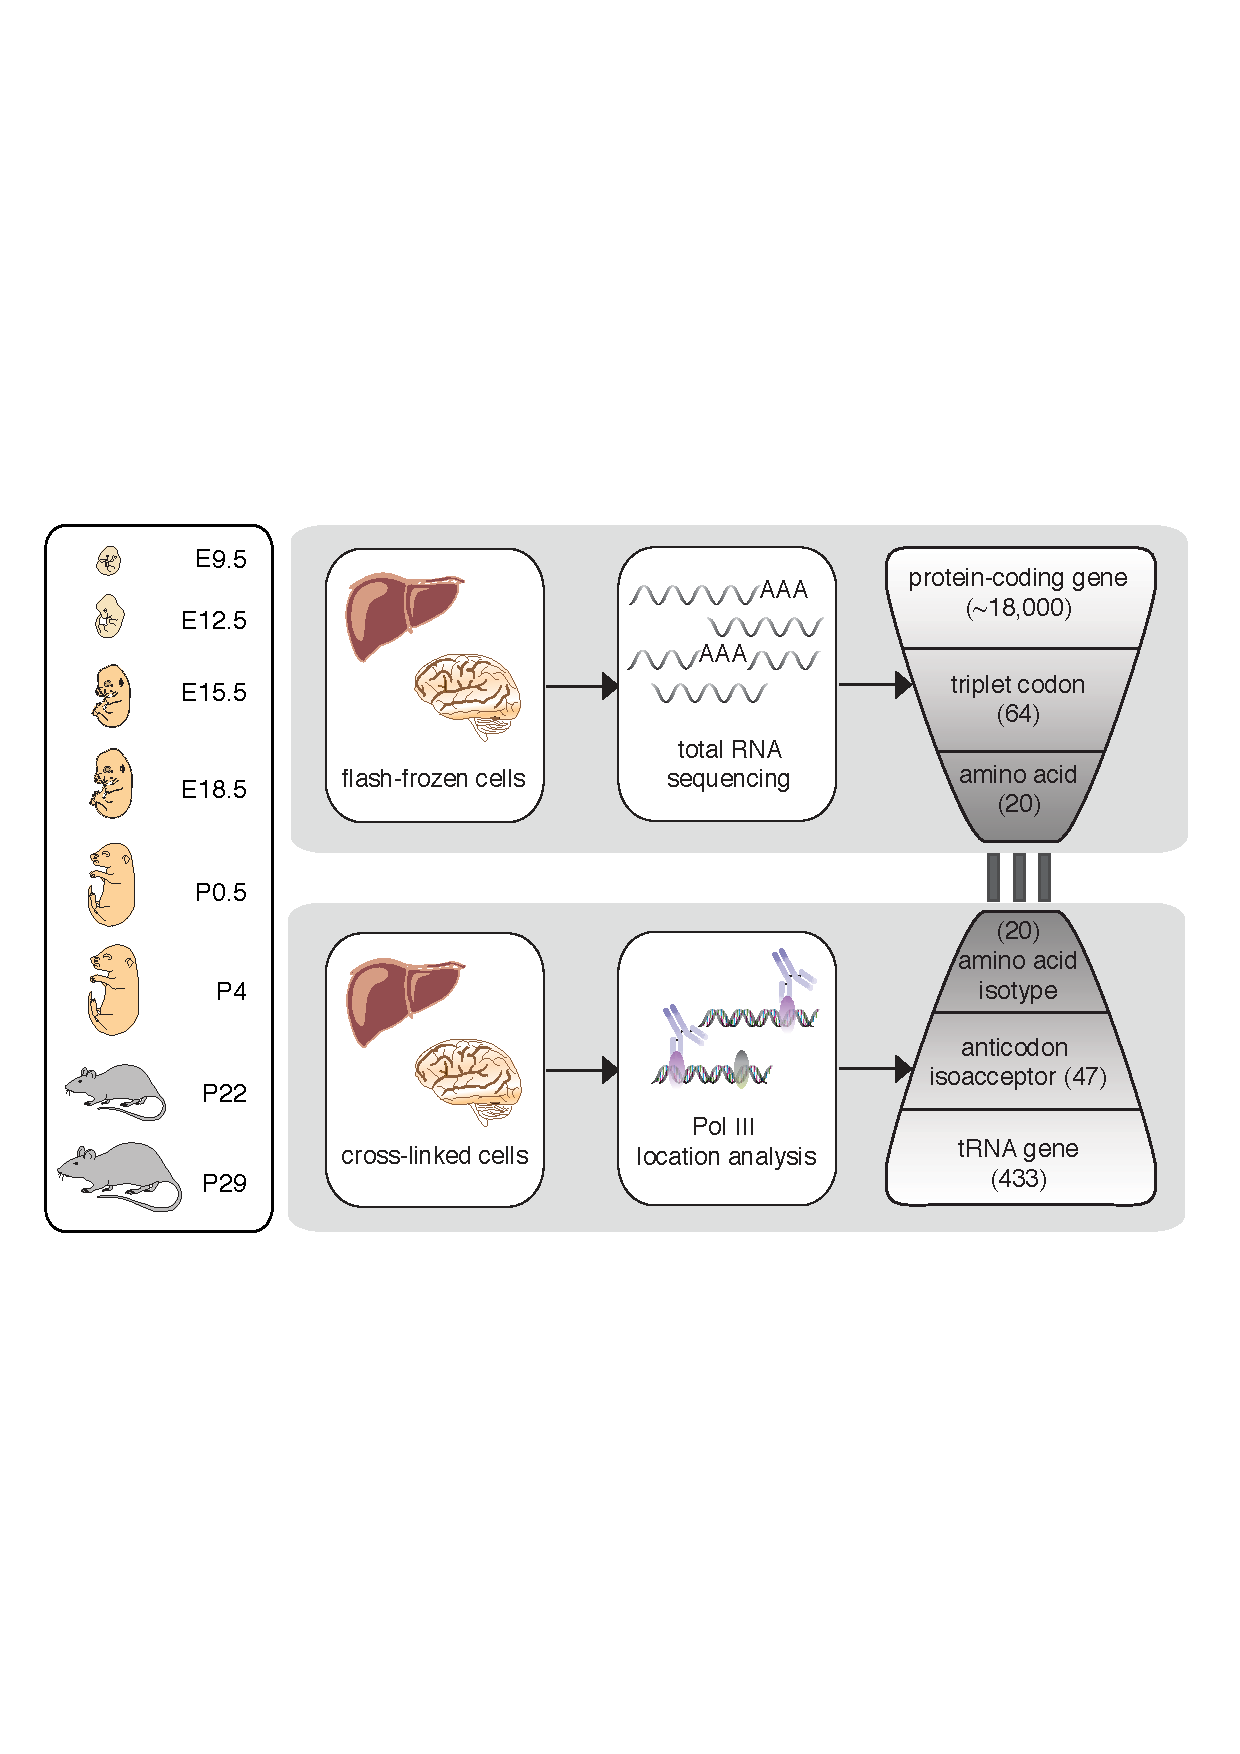
\includegraphics[width=0.8\textwidth]{trna-project-outline}
    \figcap{trna-project-outline}{Sample analysis outline}
        {Samples were collected in eight distinct time points …}
\end{figure}

In addition to the six time points described above, tissue was also collected at
two earlier stages, E9.5 and E12.5. Unfortunately, the embryo at such early
stages of development are too small to permit collecting enough tissue-specific
material. For that reason, we used the whole embryo at E9.5 and separated the
E12.5 embryo into torso and upper body.

The subsequent analysis was performed on the six later stages in liver and
brain, unless noted otherwise.

The results presented in this chapter are published as \citet{Schmitt:2014}.

%\section{Mouse tissue development as a model system to study mRNA and tRNA gene
%regulation}

\section{Protein-coding gene expression changes dynamically during mouse
development}

Changes in the expression of protein-coding genes, leading to changes in
abundance of proteins, are known to drive cellular behaviour\todo{ref}. Our data
confirms that tissue development in mice is accompanied by large-scale changes
to the \mrna transcriptome (\cref{fig:mrna-expression-change}).

A more systematic analysis shows that changes in gene expression happen
incrementally across the profiled stages of development: both in variance
(\cref{fig:mrna-pca}) and in the number of differentially expressed genes
between stages (\cref{fig:mrna-de-matrix}).

These patterns are noteworthy because they recapitulate tissue identity and
linear progression through the stages of tissue development. But they are not
particularly surprising: after all, cell function is dictated by specific
protein abundance and thus protein-coding gene transcription --- the patterns of
gene expression similarity shown in the \pca therefore recapitulate the expected
changes in cell function between tissues, and over the course of development.

\textfloat{mrna-expression-change}{spill}{%
    \centering
    \begingroup
        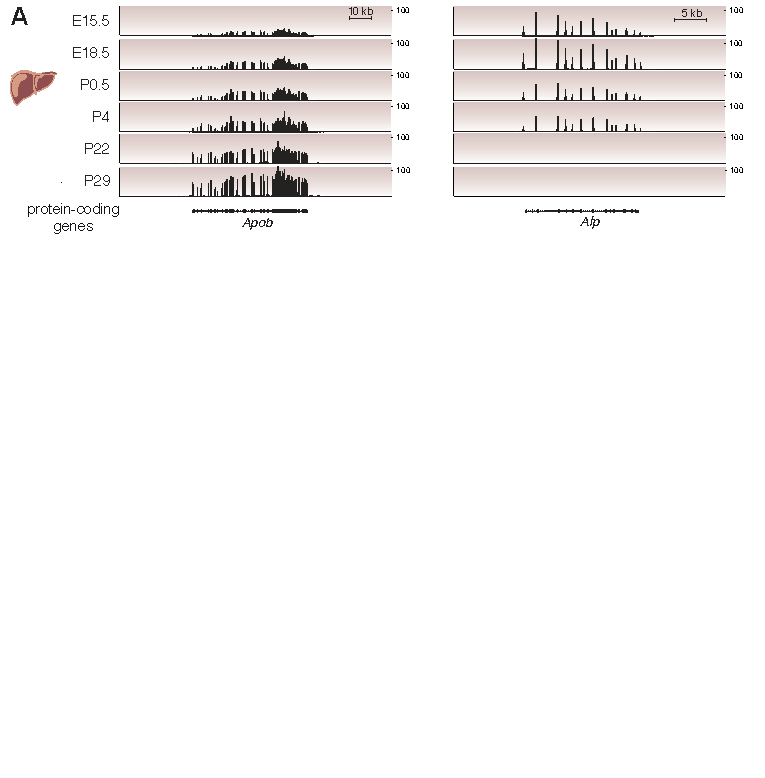
\includegraphics[width=\textwidth]{liver-mrna-expression-change}
        \subcaption{Gene expression changes of \gene{Apob} and \gene{Afp}.}
    \endgroup
    \par
    \begingroup
        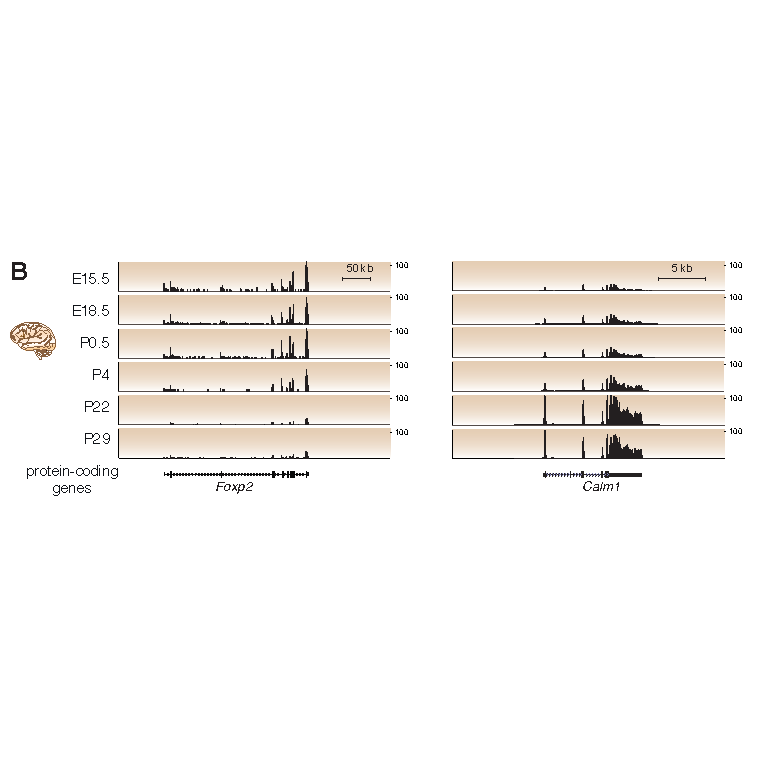
\includegraphics[width=\textwidth]{brain-mrna-expression-change}
        \subcaption{Gene expression changes of \gene{Foxp2} and \gene{Calm1}.}
    \endgroup}
    {Example of gene expression changes in development.}
    {The four genes are representative for tissue- and stage-specific genes,
    whose expression changes drive cell function. These changes can go up or
    down over the course of development, correspoding to either an up- or
    downregulation.}

\textfloatbare{spill}{%
    \begin{minipage}{0.55\textwidth}
        \centering
        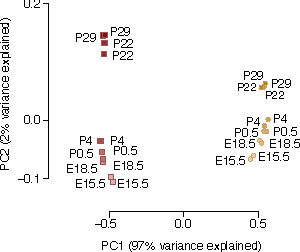
\includegraphics[width=\textwidth]{mrna-pca}
        \figcap{mrna-pca}{\pca of \mrna genes.}
            {Rotations \num{1} and \num{2} of the correlation matrix of
            protein-coding gene expressions. The percentage on the axes shows
            the amount of variance explained by each rotation.}
    \end{minipage}
    \hspace{0.1\textwidth}%
    \begin{minipage}{0.55\textwidth}
        \centering
        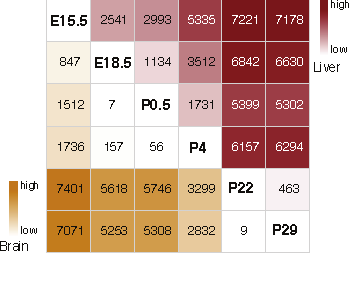
\includegraphics[width=\textwidth]{mrna-de-matrix}
        \figcap{mrna-de-matrix}
            {Number of differentially expressed \mrna genes between stages:}
            {Each off-diagonal square shows the number of differentially
            expressed genes (at a significance threshold of \(p<0.01\)) between
            the two indicated developmental stages.}
    \end{minipage}}

\section{Dynamic changes of tRNA gene expression during mouse development}

Unlike protein-coding genes, \trna genes are not directly implicated in changes
of cellular function. We therefore do not expect many changes of the levels of
\trna gene expression over the course of development. Consistent with that, we
observe that many \trna gene expression levels remain stable
(\cref{fig:trna-counts}). However, we \emph{do} observe that around \num{50}
percent of all \trna genes are differentially expressed. One specific example of
this is shown in \cref{fig:liver-trna-expression-change}.

\textfig{trna-counts}{body}{0.5\textwidth}
    {Overview over \trna gene expression change.}
    {Bar plots show different types of \trna gene expression dynamics: \trna
    genes without change in their expression levels, \trna genes with changes to
    their expression levels, which are nevertheless expressed in all stages of
    development across both tissues; and \trna genes which are only expressed in
    a subset of all conditions.}

\textfig{liver-trna-expression-change}{body}{0.5\textwidth}
    {Example of dynamically changing \trna genes.}
    {Genomic region showing different types of \trna gene expression behaviour;
    the label colours on the x axis corresponds to the colours in
    \cref{fig:trna-counts}}

Surprisingly, the \trna gene expression differences follow similar patterns as
those observed in \mrna genes \todo{fig-ref} but unlike those, they are not
readily explainable by the physiological changes to the cell; something else
needs to account for the changes.

Our first suspicion was that changes in \mrna gene expression might lead to
changes in codon demand, since different protein-coding genes are made up from
different codons. The change in codon demand in turn could lead to a change in
anticodon supply in the form of differential \trna gene expression. This would
meet the need for efficient translation: mismatching codon and anticodon pools
would either lead to a wasteful over-production of \trna[s] of a given
anticodon, or to a bottleneck in such an anticodon supply, causing efficiency
loss in translation. Both scenarios present a non-optimal scenario for the
fitness of the cell and should reasonably be selected against.

We therefore went on to quantify the codon pool corresponding to each given
transcriptome\footnote{I shall refrain from using the term “codome” to refer to
the -ome of codons}, as well as the pool of available \trna genes, grouped by
their anticodon isoacceptor identity.


\section{Every mouse mRNA transcriptome encodes the same distribution of
triplet codons and amino acids}

\section{Stable isoacceptor anticodon abundance through development indicates
tight regulation of tRNA gene expression}

\section{mRNA triplet codon usage is highly correlated with tRNA anticodon
isoacceptor abundance during development}

\section{tRNA anticodon isoacceptor families are transcriptionally compensated
across development}
